% !TEX root=/home/tavant/these/manuscript/src/manuscript.tex


\section{Polytropic index in the \ac{HET} \ac{PIC} simulations}
\label{sec-PIC_poly}

We have developed in \cref{ch-3} a sheath model that uses a polytropic state law for the electrons instead of the usual isothermal approximation.
This model successfully reproduced the sheath characteristics  when no secondary electron emission where present (fully absorbing walls).
We now include the effects of the electron emission from the wall.

In this chapter, the \ac{PIC} simulations are the same as in \cref{sec-see}. 
Hence, the dielectric electrostatic boundary condition is not modeled, but instead the walls are grounded.
In addition, we recall that the axial convection is model using Lafleur's model of convection, as discussed in \cref{sec-reinjectionnoise}.

\subsection{Polytropic index determination from the PIC simulations} \label{subsec-fluid_see_polyfit}

As previously done, we uses the mean values of the electron density $n_e$ and the electron pressure $ p_e = n_e T_e$ to find the value of the polytropic index.
\Cref{fig-radial_profiles_see} shows the radial profiles of the electron density and temperature for different values of the cross-over energy $\crover$.
The three values of $\crover$ are representative of the behaviour observed.
Indeed, $\crover=200\,\volt$ and $\crover=50\,\volt$ correspond to the upper and lower limits of regime {\bf III}, corresponding to low emission rate $\rate$, while regime {\bf I} corresponds to the case $\crover=10\,\volt$.
Regime {\bf II} is not presented has the oscillating nature of the sheath is not taken into account by the stationary sheath modeled developed here. 


\begin{figure}[hbtp]
  \centering
  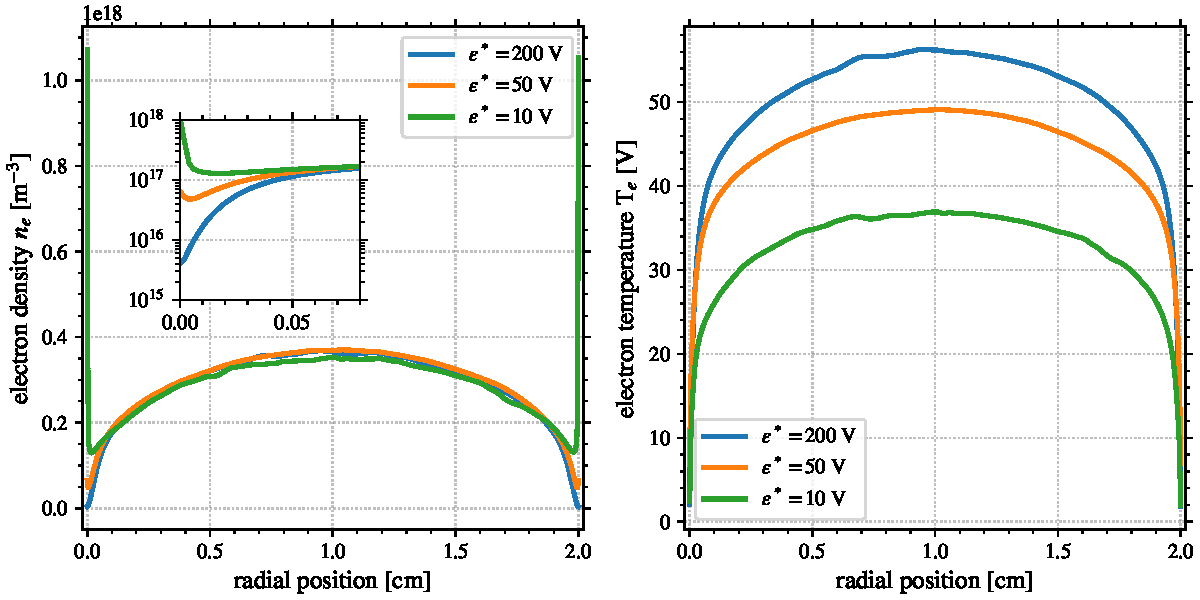
\includegraphics[width=\textwidth]{ne_Te_profiles.pdf}
  \caption{Radial profiles of (left) the electron density and (right) the electron temperature, for different values of $\crover$. The variables are averaged over the azimuthal direction and in time between $t=5\,\micro\second$ and $t=10\,\micro\second$.  }
  \label{fig-radial_profiles_see}
\end{figure}

We can see that the electron temperature presents a monotonic profile for all the values of $\crover$.
However, the electron density is not monotonic, but instead presents an increase close to the wall.
This is clearly visible in \cref{fig-log_pe-ne} that presents the electron pressure $p_e$ as a function of the electron density $n_e$, in log scale.
We see that close to the wall, where the electron pressure is the lowest, the curves present an inversion, in contrast with the case without electron emission seen in \cref{fig-polyFit}.
Otherwise in the rest of the domain, the curves are almost linear, corresponding to a polytropic law.

\begin{figure}[hbtp]
  \centering
  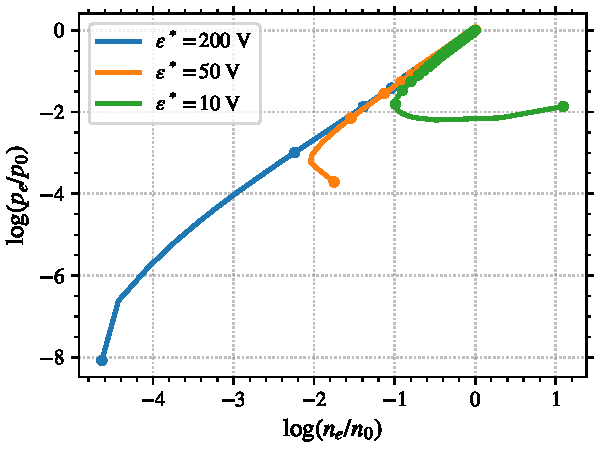
\includegraphics[width=\defaultwidth]{SEE_polytropic_presheath_and_sheath.pdf}
  \caption{Electron pressure as a function of the electron density normalized by the center variable, in log scale. The data corresponds to the same as \cref{fig-radial_profiles_see}. Markers are used every 10 cells (corresponding to around one Debye length $\lde$)}
  \label{fig-log_pe-ne}
\end{figure}

We compute the value of the polytropic index $\gamma$ from the \ac{PIC} simulations with a least mean square linear regression.
The results of the regressions are displayed in \cref{fig-polyfit_see}.
We can see that the value of $\gamma$ do not evolve significantly in regime {\bf III}, as it evolves from $\gamma=1.35$ for $\crover=200\,\volt$ to $\gamma=1.37$ for $\crover=200\,\volt$.
For $\crover=10\,\volt$, the value of the polytropic index, in the linear stage, is $\gamma=1.59$, which is not so different from regime {\bf III}.

Consequently, we can suppose that the polytropic index in the \ac{PIC} simulation with secondary electron emission is constant, and equals $\gamma=1.36$.
This value will be used in the next sections to compare the \ac{PIC} results with a fluid model of the sheath.

\renewcommand\subfigurewidth{3in}

\begin{figure}[hbtp]
  \centering
  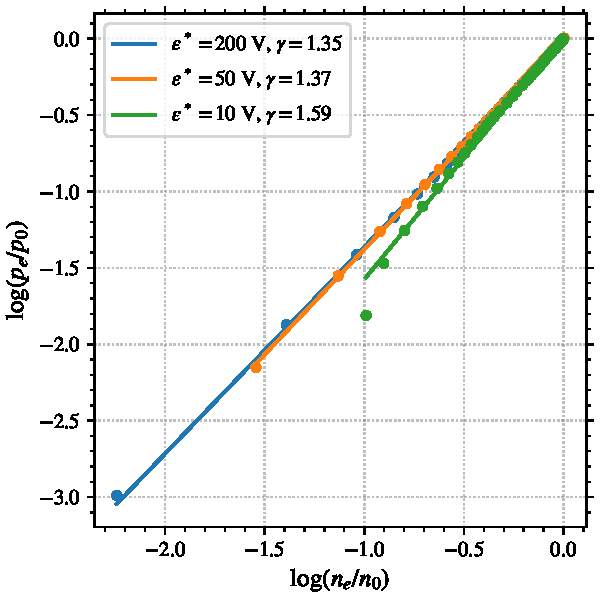
\includegraphics[width=\defaultwidth]{SEE_polyfit}
  \caption{Polytropic fit for different values of $\crover$, in the same conditions that \cref{fig-log_pe-ne}, but the last 10 cells near the wall are removed, the value of $\gamma$ fitted on the \ac{PIC} simulation data is given in the legend.}
  \label{fig-polyfit_see}
\end{figure}


\subsection{Evolution of the electron distribution function} \label{subsec-EVDF_see_polyfit}

\Cref{fig-evdf_epsstar} presents the electron distribution functions measured at the center of the simulation. \unsure{Is it the center or the sheath-edge ?}
We can see that the \ac{EVDF} presents similar profiles for the three cases, except for the mean energy that decreases with increasing value of $\crover$.

We can note that no beam is present here, even in the case of very large electron emission at $\crover=10\,\volt$, in contrast with observations of \ac{1D} PIC simulations \citep{sydorenko2006b,sydorenko2007} but in agreement with the \ac{2D} results of \citet{heron2013}.



\begin{figure}[hbtp]
  \centering
  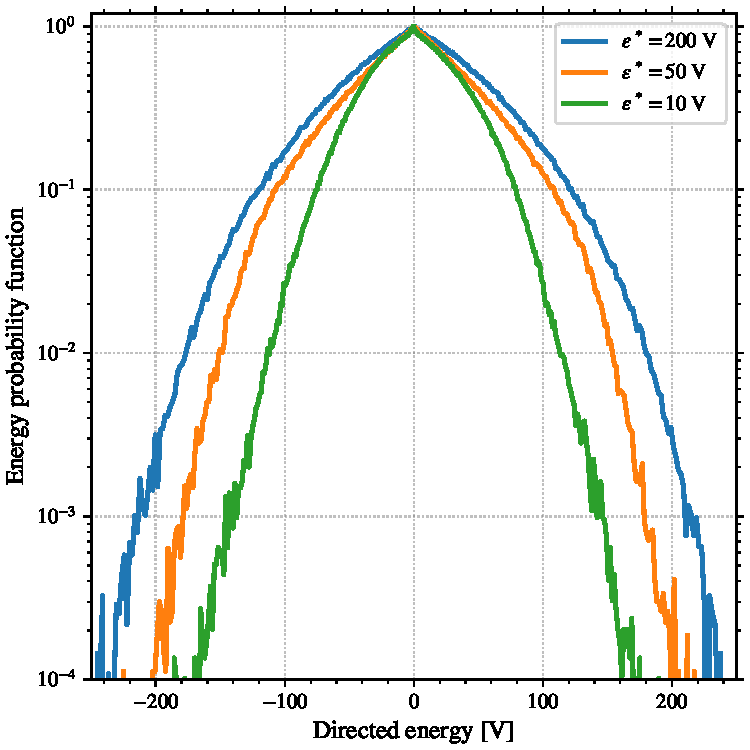
\includegraphics[width=\defaultwidth]{EVDF_Bulk.pdf}
  \caption{Electron velocity distribution function at the center of the simulation, for different values of $\crover$.}
  \label{fig-evdf_epsstar}
\end{figure}

Using the solution of the stationary Vlasov equation \cref{eq-sol}, we compute the evolution of the density and temperature of the electron population going toward the wall.
The results is compared to the mean density and temperature measured in the \ac{PIC} simulations in \cref{fig-evdf_polyfit}.

\begin{figure}[hbtp]
  \centering
  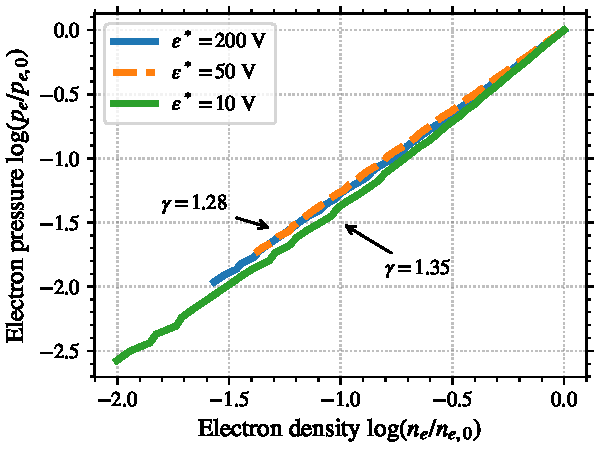
\includegraphics[width=\defaultwidth]{polyfit_evdf}
  \caption{Pressure and density in log scale of (orange) the forward electron using the stationary Vlasov equation, compared with (blue) the values measured in the \ac{PIC} simulations, for $\crover=200\,\volt$. Different polytropic models are given as well (the isothermal corresponds to $\gamma=1$).}
  \label{fig-evdf_polyfit}
\end{figure}

We can see that the pressure of the forward electron population decreases slower than the total electrons.
The may be due to the partial absorption and emission of secondary electrons at the wall, injected at $\Tsee=2\,\volt$.
Hence, we can expect that the emission rate $\sigma$, which directly depends on the forward electron population, to be better decreased with the polytropic index computed in \cref{fig-evdf_polyfit} than in \cref{subsec-fluid_see_polyfit}.

